\chapter{Computing $G_{ij}$'s and $K_{i}$}

\section{$G_{ij}$}

To compute $G_{ij}$ we first compute $F_{ij}$. $F_{ij}$ is the face containing origin in the overlay of polygons $P_{i}$ and $P_{j}$.
The following diagram taken from \cite{key1} demonstrates the notation and the construction.

\begin{figure}[h]
\begin{center}
\scalebox{0.40}{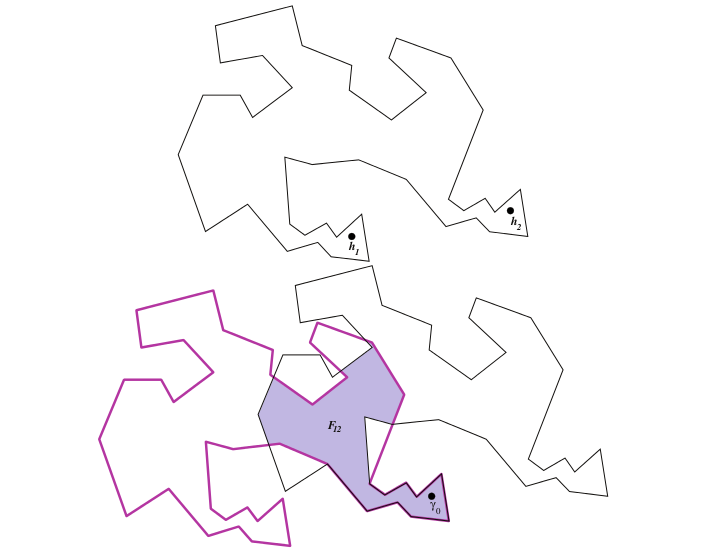
\includegraphics{Images/F12.png}}
\caption{\label{fig:Construction}$F_{12}$}
\end{center}
\end{figure}

We state without proof the following lemma. For proof please refer \cite{key1}
\begin{lemma}
 The face $F_{ij}$ has at most $2n$ edges.
\end{lemma}

Each of the $O(n)$ edges on the boundary of $F_{ij}$ can be one of three types.
\begin{enumerate}
 \item 
$e$ lies on the boundary of $P_{j}$ but not on $P_{i}$
 \item 
$e$ lies on the boundary of $P_{i}$ but not on $P_{j}$
 \item 
$e$ lies on the boundary of both $P_{j}$ and $P_{i}$

\end{enumerate}

To obtain $G_{ij}$ from $F_{ij}$ we draw visibility polygon of type 1 and type 2 edges and take their lower envelope.

\begin{figure}[h]
\begin{center}
\scalebox{0.40}{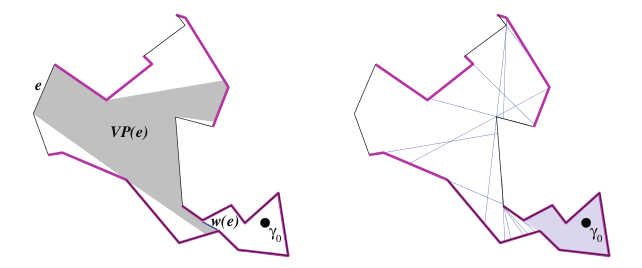
\includegraphics{Images/LowerEnvelope.png}}
\caption{\label{fig:Construction}Lower Envelope}
\end{center}
\end{figure}

Finding the lower envelope is easy using the CGAL's inbuilt Arrangement class. We find the visibility polygon of each edge of type 1
or type 2 and insert it into an arrangement. Later we check the face which contains the point $\gamma_{0}$. This face is nothing else
but $G_{ij}$
The above algorithm is repeated to obtain $G_{i1}$, $G_{i2}$, $G_{i3}$, $G_{i4}$, .... $G_{ik}$.


\section{$K_{i}$}
 To obtain $K_{i}$ we construct the 
majority rule map of all $G_{ij}$'s. $K_{i}$ is a region of special interest because of the special following special property. For 
proof of it, please refer \cite{key1}
\begin{remark} 
 A robot initially located at $h_{i}$ half localizes if it crosses the boundary of $K_{i}$.
\end{remark}




